\documentclass{article}

% if you need to pass options to natbib, use, e.g.:
%     \PassOptionsToPackage{numbers, compress}{natbib}
% before loading neurips_2020

% ready for submission
% \usepackage{neurips_2020}

% to compile a preprint version, e.g., for submission to arXiv, add add the
% [preprint] option:
\usepackage[preprint]{neurips_2020}
\bibliographystyle{unsrtnat}

% to compile a camera-ready version, add the [final] option, e.g.:
%     \usepackage[final]{neurips_2020}

% to avoid loading the natbib package, add option nonatbib:
%     \usepackage[nonatbib]{neurips_2020}

\usepackage[utf8]{inputenc} % allow utf-8 input
\usepackage[T1]{fontenc}    % use 8-bit T1 fonts
\usepackage{graphicx}
\usepackage{hyperref}       % hyperlinks
\usepackage{url}            % simple URL typesetting
\usepackage{booktabs}       % professional-quality tables
\usepackage{amsmath}
\usepackage{amssymb}
\usepackage{amsfonts}       % blackboard math symbols
\usepackage{nicefrac}       % compact symbols for 1/2, etc.
\usepackage{microtype}      % microtypography
\usepackage{alltt}
\usepackage{listings}
\usepackage{array}
\usepackage[noline, titlenumbered, vlined]{algorithm2e}
\usepackage{lmodern}
\usepackage{caption}
\usepackage{subcaption}
\usepackage{xcolor}
\SetKwComment{Comment}{$\triangleright$\ }{}
\newcommand\mycommfont[1]{\footnotesize\ttfamily\textcolor{gray}{#1}}
\SetCommentSty{mycommfont}
\SetKwBlock{Repeat}{Repeat}{end}

\newcommand{\secref}[1]{Section~\ref{#1}}
\renewcommand{\eqref}[1]{Equation~\ref{#1}}
\newcommand{\tblref}[1]{Table~\ref{#1}}
\newcommand{\figref}[1]{Figure~\ref{#1}}
\newcommand{\thmref}[1]{Theorem~\ref{#1}}
\newcommand{\algref}[1]{Algorithm~\ref{#1}}
\newcommand{\funref}[1]{Function~\ref{#1}}
\newcommand{\listingref}[1]{Listing~\ref{#1}}

\newcommand{\eg}{{\em e.g.}}
\newcommand{\ith}{$i^{th}$}
\newcommand{\cut}[1]{}
\newcommand{\todo}[1]{{\bf\em TODO:} {{\color{red}{#1}}}}

\newcommand{\spd}{\fontfamily{cmr}\textsc{\small StratPD}}
\newcommand{\cspd}{\fontfamily{cmr}\textsc{\small CatStratPD}}
\newcommand{\xnc}{${\bf X}_{\overline{c}}$}
%\newcommand{\xnj}{${\bf X}_{\overline{j}}$}
\newcommand{\Xnj}{${\bf X}_{\texttt{\char`\\}j}$}
\newcommand{\xnj}{$x_{\texttt{\char`\\}j}$}
\newcommand{\xnC}{$x_{\overline{C}}$}
\renewcommand{\xi}{x^{(i)}}
\newcommand{\yi}{y^{(i)}}
\DeclareMathOperator{\Ex}{\mathbb{E}}


%\setlist[enumerate]{itemsep=-1mm}

\title{Technical Report:\\
Partial Dependence without Model Predictions through Stratification}

\author{%
  Terence Parr \\
  University of San Francisco\\
  \texttt{parrt@cs.usfca.edu} \\
  \And
  James D. Wilson \\
  University of San Francisco\\
  \texttt{jdwilson4@usfca.edu} \\
}

\begin{document}

\maketitle

\begin{abstract}
\end{abstract}

\section{Introduction}

Partial dependence, the isolated effect of a specific variable or variables on the response variable, $y$, is important to researchers and practitioners in many disparate fields such as medicine, business, and the social sciences. For example, in medicine, researchers are interested in the relationship between an individual's demographics or clinical features and their susceptibility to illness. Business analysts at a car manufacturer might need to know how changes in their supply chain are affecting defect rates. Climate scientists are interested in how different atmospheric carbon levels affect temperature.

For an explanatory matrix, $\bf X$, with a single variable, $x_1$, a plot of the $y$ against $x_1$ visualizes the marginal effect of feature $x_1$ on $y$ exactly. Given two or more features, one can similarly plot the marginal effects of each feature separately, however, the analysis is complicated by the interactions of the variables.   Variable interactions, codependencies between features, result in marginal plots that do not isolate the specific contribution of a feature of interest to the target. For example, a marginal plot of sex (male/female) against body weight would likely show that, on average, men are heavier than women. While true, men are also taller than women on average, which likely accounts for most of the difference in average weight. It is unlikely that two ``identical'' people, differing only in sex, would be appreciably different in weight.  

Rather than looking directly at the data, there are several partial dependence techniques that interrogate fitted models provided by the user: Friedman's original partial dependence (which we will denote FPD) \citet{PDP}, functional ANOVA \citet{fanova}, Individual Conditional Expectations (ICE) \citet{ICE}, Accumulated Local Effects (ALE) \citet{ALE}, and most recently SHAP \citet{shap}.  Model-based techniques dominate the partial dependence research literature because interpreting the output of a fitted model  has several advantages. Models have a tendency to smooth over noise. Models act like analysis preprocessing steps, potentially reducing the computational burden on model-based partial dependence techniques; e.g., ALE is $O(n)$ for the $n$ records of $\bf X$. Model-based techniques are typically model-agnostic, though for efficiency, some provide model-specific optimizations, as SHAP does. Partial dependence techniques that interrogate models also provide insight into the models themselves; i.e., how variables affect model behavior.  It is also true that, in some cases, a predictive model is the primary goal so creating a suitable model is not an extra burden.

Model-based techniques do have two significant disadvantages, however. 
The first relates to their ability to tease apart the effect of codependent features because models are required to extrapolate into regions of sparse or nonexistent support; e.g., see discussions in \cite{ALE} and \cite{fanova}.  As we demonstrate in \secref{sec:experiments}, using synthetic and real data sets, model-based techniques can vary in their ability to isolated variable effects in practice.  Second, recall that there are vast armies of business analysts and scientists at work that need to analyze data, in a manner akin to exploratory data analysis (EDA), that have no intention of creating a predictive model.  Either they have no need, perhaps needing only partial dependence plots, or they do not have the expertise to choose, tune, and assess models (or write software at all).

\begin{figure}
\begin{center}
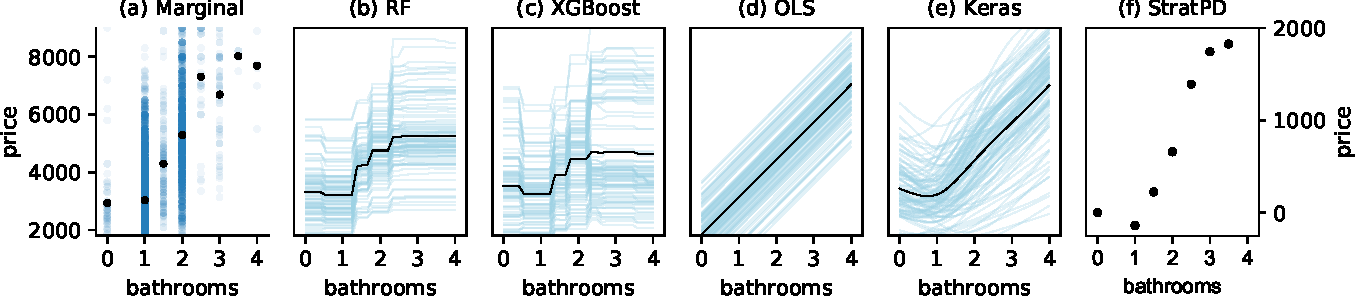
\includegraphics[scale=0.61]{images/bathrooms_vs_price.pdf}
\caption{\small Plots of bathrooms versus rent price using New York City apartment rent data. (a) marginal plot, (b) PD/ICE plot derived from random forest, (c) PD/ICE plot derived from gradient boosted machine, and (d) PD/ICE plot derived from ordinary least squares regression; sample size is 10,000 observations of \textasciitilde50k. The PD/ICE plots are  different for the same data set, depending on the chosen user model. X['bathrooms'].unique() shows (array([0. , 1. , 1.5, 2. , 2.5, 3. , 3.5, 4. ]),
 array([  54, 8151,  140, 1539,   39,   67,    3,    7])). \spd{} has missing last value, not enough data. what are $R^2$ values. how tuned all but last share y with left \vspace{-7mm}}
\label{fig:baths_price}
\end{center}
\end{figure}

Even in the case where a machine learning practitioner is available to create a fitted model for the analyst, hazards exist. First, if a fitted model is unable to accurately capture the relationship between features and $y$ accurately, for whatever reason, then partial dependence does not provide any useful information to the user.  To make interpretation more challenging, there is no definition of ``accurate enough.'' Second, given an accurate fitted model, business analysts and scientists are still peering at the data through the lens of the model, which can distort partial dependence curves. Separating visual artifacts of the model from real effects present in the data requires expertise in model behavior (and optimally in the implementation of model fitting algorithms). 

Consider the combined FPD/ICE plots shown in \figref{fig:baths_price} derived from several models (random forest, gradient boosting, linear regression, deep learning) fitted to the same New York City rent data set \citet{rent}.  The subplots in \figref{fig:baths_price}(b)-(e)  present starkly different partial dependence relationships and it is unclear which, if any, is correct.  The marginal plot, (a), drawn directly from the data shows a roughly linear growth in price for a rise in the number of bathrooms, but this relationship is biased because of the dependence of bathrooms on other variables, such as the number of bedrooms. (e.g., five bathroom, one bedroom apartments are unlikely.)  For real data sets with codependent features, the true relationship is unknown so it is hard to evaluate the correctness of the plots. (Humans are unreliable estimators, which is why we need data analysis algorithms in the first place.) Nonetheless, having the same algorithm, operating on the same data, give meaningfully different partial dependences is undesirable and makes one question their validity.

Experts are often able to quickly recognize model artifacts, such as the stairstep phenomenon inherent to the decision tree-based methods in \figref{fig:baths_price}(b) and (c).  In this case, though, the stairstep is more accurate than the linear relationship in (d) and (e) because the number of bathrooms is discrete (except for ``half baths'').  The point is that interpreting model-based partial dependence plots can be misleading, even for experts. 

An accurate mechanism to compute partial dependences that did not peer through fitted models would be most welcome.  Such partial dependence curves would be accessible to users, like business analysts, who lack the expertise to create suitable models and would also reduce the chance of plot misinterpretation due to model artifacts. The curves could also help machine learning practitioners to choose appropriate models based upon relationships exposed in the data.

In this paper, we propose a strategy, called {\textsc{strat}ified \textsc{p}artial \textsc{d}ependence} (\spd{}), that ({\it i}) computes partial dependences directly from training data $({\bf X}, {\bf y})$, rather than through the predictions of a fitted model, and ({\it ii}) does not presume mutually-independent features.  As an example, \figref{fig:baths_price}(f) shows the partial dependence plot computed by \spd. The technique depends on the notion of an idealized partial dependence:  integration over the partial derivative of $y$ with respect to the variable of interest for the smooth function that generated $({\bf X}, {\bf y})$. As that function is unknown, we estimate the partial derivatives from the data non-parametrically.  Colloquially, the approach examines changes in $y$ across $x_j$ while holding \xnj{} constant or nearly constant (\xnj{} denotes all observations with all variables except $x_j$). A similar stratification approach works for categorical variables (\cspd). Both \spd{} and \cspd{} are quadratic in $n$, in the worst case (like FPD), but \spd{} behaves linearly on real data sets.  Our prototype is currently limited to regression, isolates only single-variable partial dependence, and cannot identify interaction effects (as ICE can).  The software is available via Python package {\tt stratx} with source code at {\tt github}, including the code to regenerate images in this paper.

We begin by describing the proposed stratification approach in \secref{sec:stratpd} then compare \spd{} to related (model-based) work in \secref{sec:related}. In \secref{sec:experiments}, we present partial dependence curves generated by \spd{} and \cspd{} on real data sets, contrast the plots with those of existing methods, and use synthetic data to highlight possible bias in some model-based methods.

% ------------------------------------------------------------------------------------------------------------------------------------
\section{Partial dependence without model predictions}\label{sec:stratpd}

In special circumstances, we know the precise effect of each feature $x_j$ on $y$.  Assume we are given training data pair ($\bf X, y$) where ${\bf X} = [x^{(1)}, \ldots, x^{(n)}]$ is an $n \times p$ matrix whose $p$ columns represent observed features and ${\bf y}$ is the $n \times 1$ vector of responses. For any smooth function $f:\mathbb{R}^{p} \rightarrow \mathbb{R}$ that precisely maps each $\xi$ vector to response $y^{(i)}$, ${y^{(i)}} = f(\xi)$, the partial derivative of $y$ with respect to $x_j$ gives the change in $y$ holding all other variables constant.  Integrating the partial derivative then gives the {\em idealized partial dependence}  of $y$ on $x_j$, the isolated contribution of $x_j$ to $y$:

\noindent {\bf Definition 1} The {\em idealized partial dependence} of $y$ on feature $x_j$ for smooth generator function $f:\mathbb{R}^{p} \rightarrow \mathbb{R}$ evaluated at $x_j = z$ is the cumulative sum up to $z$ \todo{do we need to say that the partial derivative is continuous also?}:

\begin{equation}\label{eq:pd}
\text{\it PD}_j(z) = \int_{min(x_j)}^z \frac{\partial f}{\partial x_j} dx_j
\end{equation}

$\text{\it PD}_j(z)$ is the value contributed to $f$ by $x_j$ at $x_j = z$ and $\text{\it PD}_j(min(x_j))=0$. The advantages of this definition are that it does not depend on predictions from a fitted model and is insensitive to codependent features.  Although the underlining generator function is unknown, we can estimate its partial derivatives from the raw training data. ALE also derives partial dependence by estimating and integrating across partial derivatives (e.g., see Equation 7 in \cite{ALE}) but does so using local changes in fitted model predictions.

The key idea is to stratify \xnj{} feature space into disjoint regions of observations where all \xnj{} variables are approximately matched across the observations in that region. Within each \xnj{} region, any fluctuations in the response variable are likely due to the variable of interest, $x_j$.  Estimates of the partial derivative within a region are estimated discretely as the changes in $y$ values between unique and ordered $x_j$ positions:  $(y^{(i+1)} - \yi)/(x_j^{(i+1)} - x_j^{(i)})$ for all $i$ in a region.  This amounts to performing piecewise linear regression through the leaf observations, one model per unique pair of $x_j$ values, and collecting the model $\beta_1$ coefficients to estimate partial derivatives. The overall partial derivative at $x_j=z$ is the average of all slopes, found in any region, whose range $[x_j^{(i)},x_j^{(i+1)})$ spans $z$.  Stratification occurs through the use of a decision tree fit to (\Xnj, $\bf y$), whose leaves aggregate observations with equal or similar \xnj{} features. The \xnj{} features can be numerical variables or label-encoded categorical variables (assigned a unique integer). \spd{} only uses the tree for the purpose of partitioning feature space and never uses predictions from any model. See \algref{alg:StratPD} for more details.

For this approach to work, decision tree leaves must satisfactorily stratify \xnj{}. If the \xnj{} observations in each region are not similar enough, the relationship between $x_j$ and $y$   is less accurate.  Regions can also become so small that even the $x_j$ values become equal, leaving a single unique $x_j$ observation in a leaf. Without a change in $x_j$, no partial derivative estimate is possible and these nonsupporting observations must be  ignored. A degenerate case occurs when identical or nearly identical $x_j$ and $x_j'$ variables exist. Flattening $x_j$ as part of \xnj{} would also flatten $x_j'$, leading to both exhibiting flat curves, as if the decision tree were trained on $(\bf X, y)$ not (\Xnj, $\bf y$). Our experiments show that using the collection of leaves from a random forest, which restricts the number of variables available during node splitting, prevents partitioning from relying too heavily on either $x_j$ or $x_j'$. Some leaves have observations that vary in $x_j$ or $x_j'$ and partial derivatives can still be estimated. \todo{maybe talk about how PD/ICE on RF underestimates the curve.}

\spd{} uses hyper parameter {\tt\small min\_samples\_leaf} to control the minimum number of observations in each decision tree leaf.  Generally speaking, smaller values lead to more confidence that fluctuations in $y$ are due solely to $x_j$, but more observations per leaf allow \spd{} to capture more nonlinearities and make it less susceptible to noise.  As the leaf size grows, however, one risks introducing contributions from \xnj{} into the relationship between $x_j$ and $y$. At the extreme, the decision tree would consist of a single leaf node containing all observations, leading to a marginal not partial dependence curve.

\spd{} uses another hyper parameter called {\tt\small min\_slopes\_per\_x} to ignore any partial derivatives estimated with too few observations.  Dropping uncertain partial derivatives greatly improves accuracy and stability. Partial dependences computed by integrating over local partial derivatives are highly sensitive to partial derivatives computed at the left edge of any $x_j$'s range because imprecision at the left edge affects the entire curve.  This presents a problem when there are few samples with $x_j$ values at the extreme left (see, for example, the $x_j$ histogram of \figref{fig:yearmade}(d)).  Fortunately, sensible defaults for \spd{} (10 observations and 5 slopes) work well in most cases and  were used to generate all plots in this paper.

For categorical variables, \cspd{} uses the same stratification approach, but cannot apply  regression of $y$ to non-ordinal, categorical $x_j$. Instead, \cspd{} groups leaf observations by category and computes the average $\bar{y}$ per category. Then,  within each leaf, it chooses a random reference category and subtracts that category's $\bar{y}$ value from the leaf $\bar{\bf y}$ vector to get a vector of relative deltas between categories: $\Delta {\bf y}$ = $\bar{\bf y} - \bar{\bf y}_{\it refcat}$. The $\Delta  {\bf y}$ vectors from all leaves are then merged via averaging, weighted by the number of observations per category, to get the overall effect of each category on $y$.  The delta vectors for two leaves, $\Delta {\bf y}$ and $\Delta {\bf y}'$, can only be merged if there is at least one category in common.  \cspd{} initializes a running average vector to the first leaf's $\Delta  {\bf y}$ and then makes  passes over the remaining vectors, merging any vectors with a category in common with the running average vector.  Observations associated with any remaining, unmerged leaves must be ignored.

Stratification of high-cardinality categorical variables tends to create small groups of category subsets, which complicates the averaging process across groups. (Such $\Delta {\bf y}$ vectors are sparse and {\it NaN}s represent missing values.) If both groups have the same reference category, merging is a simple matter of averaging the two delta vectors, where {\it mean}({\it z,NaN}) = {\it z}.  For delta vectors with different reference categories and at least one category in common, one vector is adjusted to use a randomly-selected reference category, $c$, in common: $\Delta {\bf y}' = \Delta {\bf y}' - \Delta {\bf y}_c' + \Delta {\bf y}_c$. That equation adjusts vector $\Delta {\bf y}'$ so $\Delta {\bf y}_c'=0$ then adds the corresponding value from $\Delta {\bf y}$ so $\Delta {\bf y}_c' = \Delta {\bf y}_c$, which renders the average of $\Delta {\bf y}$ and $\Delta {\bf y}'$ meaningful.  \cspd{} uses a single hyper parameter {\tt\small min\_samples\_leaf} to control stratification. See \algref{alg:CatStratPD} for more details.

\spd{} and \cspd{} both have theoretical worst-case time complexity of $O(n^2)$ for $n$ observations. For \spd{}, stratification costs $O(p n \,log n)$, computing $y$ deltas for all observations among the leaves has linear cost, and averaging slopes across unique $x_j$ ranges is on the order of $|unique({\bf X}_j)| \times n$ or $n^2$ when all ${\bf X}_j$ are unique in the worst case. \spd{} is, thus, $O(n^2)$ in the worst case.  \cspd{} also stratifies in $O(p n \,log n)$ and computes category deltas linearly in $n$ but must make multiple passes over the $|T|$ leaves to average all possible leaf category delta vectors.  In practice, three passes is the max we have seen (for high-cardinality variables), so we can assume the number of passes is some small constant. Averaging two vectors costs $|unique({\bf X}_j)|$, so each pass requires $|T| \times |unique({\bf X}_j)|$. The number of leaves is roughly $n / {\tt\small min\_samples\_leaf}$ and, worst-case, $|unique({\bf X}_j)|=n$, meaning that merging dominates \cspd{} complexity leading to $O(n^2)$.  Experiments show that our prototype is fast enough for practical use (see \secref{sec:experiments}).

% ------------------------------------------------------------------------------------------------------------------------------------
\section{Related work}\label{sec:related}

\citet{PDP} defines the partial dependence of $\hat{f}$ on feature subsets, $S$, as an expectation conditioned on the remaining variables:

\[
{\it FPD}_S(x_S) = \Ex[\hat{f}(x_S,{\bf X}_{\texttt{\char`\\}S})] = \frac{1}{n} \sum_{i=1}^n \hat{f}(x_S, x_{\texttt{\char`\\}S}^{(i)})
\]

\cut{
\[
{\it FPD}_j(x_j=z) = \Ex[\hat{f}(x_{j}=z,{\bf X}_{\texttt{\char`\\}j})] = \frac{1}{n} \sum_{i=1}^n \hat{f}(x_j=z, x_{\texttt{\char`\\}j}^{(i)})
\]
}

\cut{
\noindent FPD replaces ${\bf X}_j$ with $z$ then computes the average model output for the altered $x^{(i)}$.
}

% ICE 

The individual conditional expectation (ICE) plot from \cite{ICE} is a local method that estimates the partial dependence of the prediction $\hat{f}$ on $x_S$, or single variable $x_j$, across individual observations. Suppose that $(x_j^{(i)}, x_{\texttt{\char`\\}j}^{(i)})$ are the values of the $i$th row of $\mathbf{X}$. For each $i$, the ICE plot produces a curve from the fitted model over all values of $x_j$ while holding \xnj{} fixed: $\hat{f}^{(i)}_j = \widehat{f}((\{x_j^{(k)}\}_{k = 1}^n, x_{\texttt{\char`\\}j}^{(i)}))$. By construction, the FPD curve for a variable $x_j$ is the average over all ICE curves for that variable. The motivation for ICE is to identify variable dependencies not shown by the FPD curve (because they average out). Typically both ICE and FPD are used to examine the partial dependence of $y$ on $x_j$. Both techniques operate by observing $\hat{f}$ output as \xnj{} (FPD) or $x_j$ (ICE) values are shifted through all $n$ observations.

% SHAP

Rather than shift feature values, SHAP from \cite{shap}, with roots in {\em Shapley regression values} \citep{shapley-regression}, calculates the average marginal effect of adding $x_j$ to models trained on all possible  subsets of features, $F$:

\[
\phi_j(\hat{f},{\bf x}) = \sum_{S \subseteq F \texttt{\char`\\} \{j\}}\
\frac{|S|!(|F|-|S|-1)!}{|F|!}\
 [ \hat{f}_{S \cup \{j\}}(x_{S \cup \{j\}}) - \hat{f}_S(x_S) ]
\]

To avoid training a combinatorial explosion of models with the various feature subsets, $\hat{f}_S(x_S)$, SHAP reuses a single model fitted to $(\bf X, y)$ by running simplified feature vectors into the model. One possible implementation for simplified vectors is to replace ``missing'' $x_j$ features with the expected value of $x_j$. SHAP uses a more general approach that approximates $\hat{f}_S(x_S)$ with $\Ex[\hat{f}(x_{S},{\bf X}_{\texttt{\char`\\} S}) | {\bf X}_S = x_S]$ where ${\bf X}$ is called the {\em background set} and users can pass in, for example, a single vector with $x_j$ averages or even the entire training set.  For efficiency reasons, SHAP's implementation (in ``interventional'' mode) approximates $\Ex[\hat{f}(x_{S},{\bf X}_{\texttt{\char`\\}S}) | {\bf X}_S = x_S]$ with $\Ex[\hat{f}(x_{S},{\bf X}_{\texttt{\char`\\} S})]$.  To further reduce computation costs, SHAP users typically explain a very small subsample of the data set, but with potentially a commensurate reduction in the explanatory resolution of the underlying population. SHAP has model-type-dependent optimizations for linear regression, deep learning, and decision-tree based models.

while the formal SHAP definition does not assume feature independence, the SHAP implementation does so for the specific purpose of simulating models trained on feature subsets. The SHAP definition approximates $\hat{f}_S(x_S)$ with $\Ex[\hat{f}(x_{S},{\bf X}_{\bar{S}}) | {\bf X}_S = x_S]$, but SHAP's implementation approximates $\hat{f}_S(x_S)$ with $\Ex[\hat{f}(x_{S},{\bf X}_{\bar{S}})]$, which requires feature independence for accuracy. \cite{janzing2019feature} argues that ``{\em unconditional} [as implemented] rather than {\em conditional} [as defined] expectations provide the right notion of dropping features.'' In practice, however, we have observed several instances of questionable SHAP partial dependence curves for features important to the model.

From a mathematical perspective, the bias is clear because $\Ex[\hat{f}(x_{S},{\bf X}_{\bar{S}})]$ is equivalent to $FPD_S(x)$ that is known to be biased by codependent features. (Equation 53 in \citealt{PDP} gives a summation equivalent to $\Ex[\hat{f}(x_{S},{\bf X}_{\bar{S}})]$)

% ALE

ALE has same goal as us. we are model-free version. both estimate partial derivatives then cumsum.  We do it point to point, they do in regions from min to max of support.  both use finite differences; ALE using finite differences on $\hat{f}$ and us on $\bf y$.  They do binning with intervals and we jump between unique $x_j$.  that means they can ask for predictions for previously unseen  $x_j$ even if within the support range.  By the way what if the support range is not a simple Gaussian density function? are we then picking values in low-density areas such as in between humps? anyway, we only consider existing values.

ALE cats appendix E: ``The main consideration for a ?reasonable? ordering is that function
extrapolation outside the data envelope should be avoided as much as possible when neighboring of values of xj are plugged into f(xj , x not j).'' ``we order the levels of Xj based on how dissimilar the sample values {xi, not j : i = 1, 2, . . . , n} are across the levels of Xj.'' ordering Boolean then has no effect since any order has the same difference between y values of true/false. $K$ set to the number of nonempty category levels. from his email: ``The way ALE plots treats categorical predictors still requires some extrapolation. With binary categorical variables, the extrapolation would be exactly the same as for PD plots. But with many categories, the extrapolation would be substantially less.''

ALE guys says ``the difference is that ALE plots hold \xnj exactly constant as it varies $x_j$ across categories, which it can do because it uses the fitted model $f(x_j, x_{ not j})$, whereas your approach keeps \xnj approximately the same as it varies $x_j$ across categories, which it must do because it does not use any fitted model.''

\begin{figure}[htbp]
\begin{center}
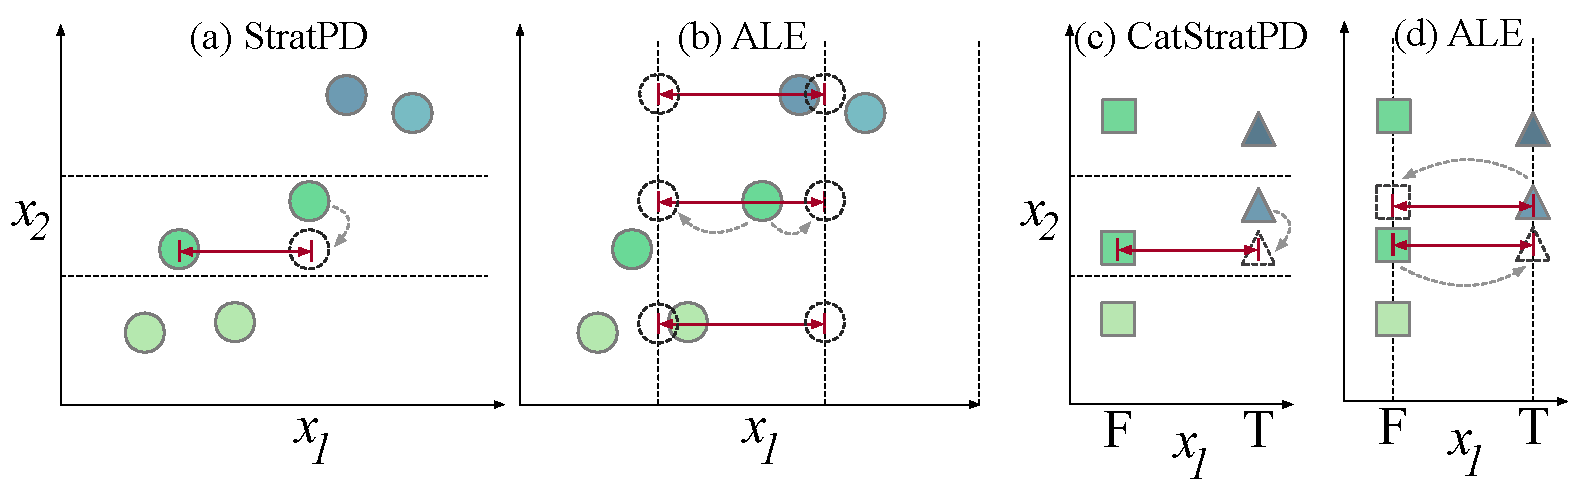
\includegraphics[scale=.4]{images/partitioning.pdf}
\caption{\small $x_2$ continuous and partitioned by decision tree fit to (\xnj, ${\bf y}$), $x_1$ continuous (a), (b) and categorical (c), (d). Small wedges on $x_1$ axis indicate PD curve points}
\label{fig:partitioning}
\end{center}
\end{figure}

if $x_2$ is also cat then assuming same value means shifting $x_2$ to new cat as well for us, right? dec trees tend to test existing values for splits so will likely keep integers in their own leaves. In the case of x2 being cat with k levels, we can use {\tt\small max\_leaf\_nodes=8, min\_samples\_leaf=1} but in general we can still shift x2 cats during strat. verified by experiment.


ALE partitions $x_j$ into bins then fixes \xnj to compute average finite difference of $y$ at $x_j=z$ in $x_j$ neighborhood (all \xnj in that $x_j$ bin) whereas we partition \xnj then compute average finite diff of $y$ at $x_j=z$ across those $p-1$ dim regions hoping they are repetitions of the same $p-1$ dimensional vector (all same).

\cut{
Third, it's reasonable to ask why we use unique $x_c$ values within each $L$ as the bin edges, rather than splitting $x_c$ into fixed-width bins.  This was our original approach because of its simplicity, but it required another hyper parameter, such as $nbins$, and led to high proportions of non-supporting observations in some data sets. When all or most of the $x_c$ values are discrete integers, some choices of $nbins$ would lead to virtually all bins in all leaves having a single $x_c$ value. Also, binning integers leads to awkward bins, such as 1.8 to 3.2 bedrooms or dayofweek 1.3 to 2.1.  Using the unique $x_c$ values themselves avoids a second hyper parameter and guarantees that bins do not have non-supporting observations unless the entire leaf has a single unique $x_c$.
}

\todo{in case of discrete...}



% COMPARE

The inner difference $\hat{f}_{S \cup \{j\}}(x_{S \cup \{j\}}) - \hat{f}_S(x_S)$ = $\Ex[\hat{f}(x_{S \cup \{j\}},{\bf X}_{\texttt{\char`\\} (S \cup \{j\})})] - \Ex[\hat{f}(x_{S},{\bf X}_{\texttt{\char`\\} S})]$ = $\text{\it FPD}_{S \cup \{j\}}({\bf x}) - \text{\it FPD}_{S}({\bf x})$

so in practice this keeps the same model but shifts feature values like FPD/ICE. SHAP also observes changes in model output for shifted feature values, but using models trained on all possible subsets, $S$, of features:


{\bf Comparison}

${\it FPD}_j(z) = \Ex[\hat{f}(x_{j}=z,{\bf X}_{\texttt{\char`\\}j})])$

SHAP for one $S$ is $\phi_j(\hat{f},{\bf x}) = \Ex[\hat{f}(x_{S \cup \{j\}},{\bf X}_{\texttt{\char`\\} (S \cup \{j\})})  | {\bf X}_{S \cup \{j\}} = x_{S \cup \{j\}}] - \Ex[\hat{f}(x_{S},{\bf X}_{\texttt{\char`\\} S})  | {\bf X}_S = x_S ]$ for all subsets $S \subset F$ for $F = \{1, 2, .., p\}$. When $S = F \texttt{\char`\\} \{j\}$, like ALE, it becomes $\Ex[\hat{f}(x_F)] - \Ex[\hat{f}(x_{F \texttt{\char`\\} \{j\}},{\bf X}_j)]$ or $\hat{f}({\bf x}) - \text{\it FPD}_{F \texttt{\char`\\} \{j\}}(x)$ if assume independence.

ALE at $x_j=z$, it is cumsum of $\Ex[\hat{f}(b_k, {\bf X}_{\texttt{\char`\\}j}) - \hat{f}(b_{k-1}, {\bf X}_{\texttt{\char`\\}j}) \, | \, x_j \in (b_{k-1},b_k]]$ for bin $b_k$ partitioning min..max for var $j$ into $K$ intervals.

StratPD at $x_j=z$ is $\Ex[ (y^{(i_L+1)} - y^{i_L})/(x_j^{(i_L+1)} - x_j^{(i_L)}) \, | \, z \in [x_j^{(i_L+1)} - x_j^{(i_L)}) \text{ and } L \in T]$





$\Ex[ \phi_j(\hat{f},x) | {\bf X}_j = z] = FPD_j(x) - \bar{y}$ if features independent. SHAP's implementation approximates $\hat{f}$ trained on just $S$ features, $\hat{f}_S(x_S)$, with $\Ex[\hat{f}(x_{S},{\bf X}_{\bar{S}})]$ by assuming independent features.

Strobl thing \cite{rfimp}: ``conditional permutation scheme, where X j is permuted only within groups of observations with Z = z, to preserve the correlation structure between X j and the other predictor variables.''  ``Our suggestion is to define the grid within which the values of X j are permuted for each tree by means of the partition of the feature space induced by that tree. The main advantages of this approach are that this partition was already learned from the data during model fitting, contains splits in categorical, ordered and continuous predictor variables and can thus serve as an internally available means for discretizing the feature space.'' 

Reviewer: ``Their motivation is to handle the same extrapolation problems caused by having to plug in nonsensical combinations of correlated predictors, which is common to PD plots and permutation based importance measures.''

cold start, counting execution time and number of hyper parameters. particularly deep learning

The techniques differ in algorithm simplicity, performance, and ability to isolate codependent variables. a nonparametric technique could also inform which machine learning model to use if a model is desired.

SHAP is mean centered FPD for independent variables, proof in supplemental material.

% ------------------------------------------------------------------------------------------------------------------------------------
\section{Experimental results}\label{sec:experiments} 

In this section, we demonstrate experimentally that \spd{} and \cspd{} compute accurate partial dependence curves for synthetic data and plausible results for a real data set. Experiments also provide evidence that existing model-based techniques can provide meaningfully-biased curves. We begin by comparing the partial dependence curves from popular techniques on synthetic data with complex interactions.

\figref{fig:interactions} illustrates that FPD, SHAP, ALE, and \spd{} all suitably isolate the effect of independent individual variables on the response for noiseless data generated via: $y = x_1^2 + x_1 x_2 + 5 x_1 sin(3 x_2) + 10$ for $x_1,x_2,x_3 \sim U(0,10)$ where $x_3$ does not affect $y$. The shapes of the curves for all techniques look similar except that \spd{} starts all curves at $y=0$ (as could the others). SHAP's curves have the advantage that they indicate the presence of variable interactions. To our eye, \spd's curves are smoothest despite not having access to model predictions.

\begin{figure}[htbp]
\begin{center}
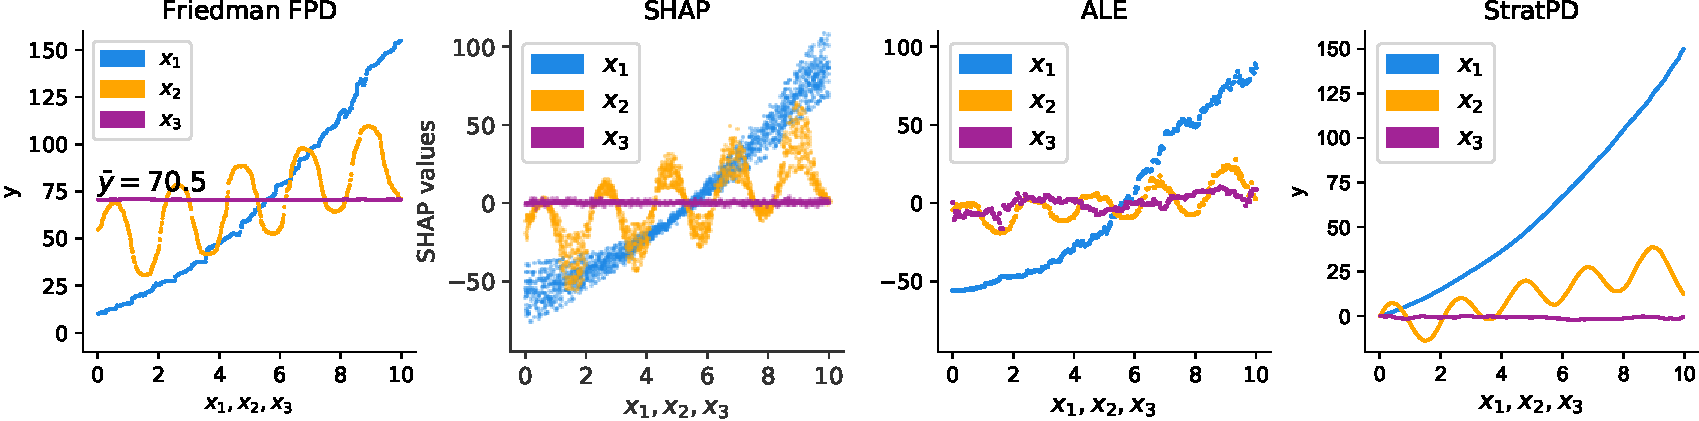
\includegraphics[scale=0.45]{images/interactions.pdf}
\caption{\small $y = x_1^2 + x_1 x_2 + 5 x_1 sin(3 x_2) + 10$ where $x_1,x_2,x_3 \sim U(0,10)$ and $x_3$ does not affect $y$. No noise added. Random forest with 10 trees. $R^2$  0.9973}
\label{fig:interactions}
\end{center}
\end{figure}

Models have a tendency to smooth out noise and a legitimate concern is that, without the benefit of a model, \spd{} could be adversely affected. \figref{fig:noise} demonstrates \spd{} curves for noisy quadratics generated from $y = x_1^2 + x_1 + 10 + \epsilon$ where $\epsilon \sim N(0,\sigma)$ $\epsilon$ and, at $\sigma=2$, 95\% of the noise falls within [0,4] (since $2\sigma = 4$), meaning that the signal-to-noise ratio is at best 1-to-1 for $x_1^2$ in $[-2,2]$. For zero-centered Gaussian noise and this data set, \spd{} accuracy is stable.  The superfluous noise variable $x_3$ in \figref{fig:interactions} also did not confuse \spd.

\begin{figure}[htbp]
\begin{center}
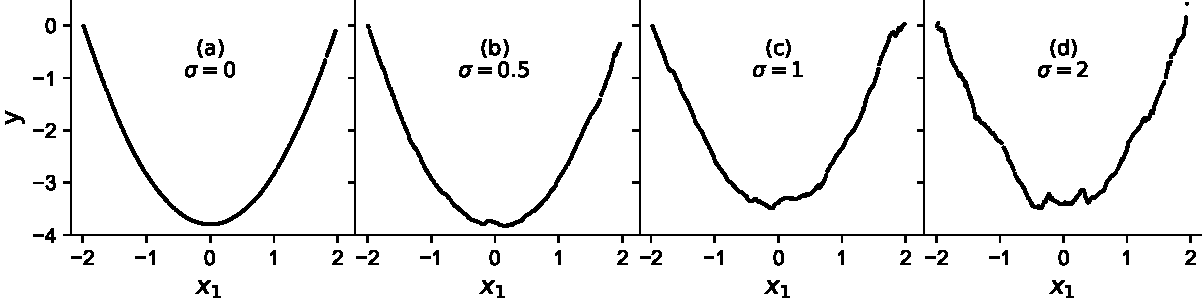
\includegraphics[scale=0.45]{images/noise.pdf}
\caption{\small $y = x_1^2 + x_1 + 10 + \epsilon$ where $x_1,x_2 \sim U(-2,2)$, $\epsilon \sim N(0,\sigma)$ with $\sigma \in [0,0.5,1,2]$.}
\label{fig:noise}
\end{center}
\end{figure}

Turning to categorical variables, \figref{fig:statetemp} presents partial dependence curves for FPD, ALE, and \cspd{} derived from a noisy synthetic weather data set, where temperature varies in sinusoidal fashion over the year and with different baseline temperatures per state. (The vertical ``smear'' in the FPD plot shows the complete sine waves but from the side, edge on.)  Variable {\tt\small state} is independent and all plots identify the baseline temperature per state correctly.

\cut{
\begin{equation}\label{eq:weather}
y = t[x_{\it state}] + 10 sin(\frac{2\pi}{365}x_{\it dayofyear}+\pi) + \epsilon, ~~~ \epsilon \sim N(0, 4)
\end{equation}
}

\begin{figure}[htbp]
\begin{center}
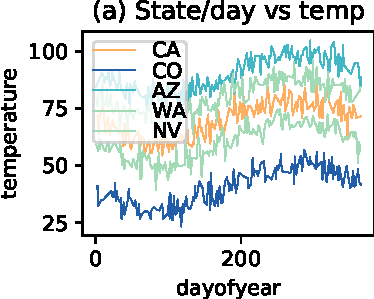
\includegraphics[scale=0.45]{images/dayofyear_vs_temp.pdf}~~
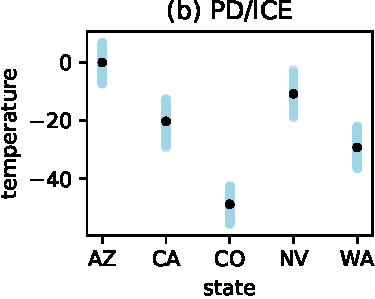
\includegraphics[scale=0.45]{images/state_vs_temp_pdp.pdf}~~
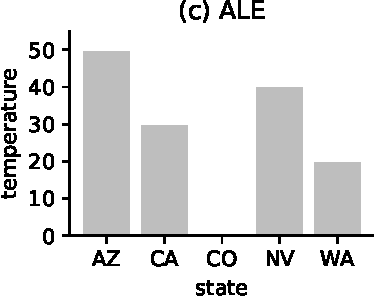
\includegraphics[scale=0.45]{images/state_ale.pdf}~~
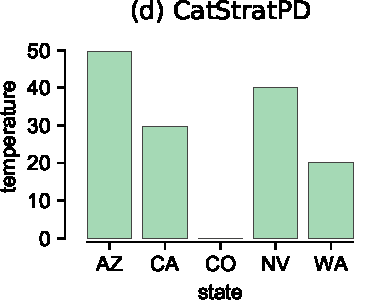
\includegraphics[scale=0.45]{images/state_vs_temp_stratpd.pdf}~~
\caption{\small $y = base[x_{\it state}] + 10 sin(\frac{2\pi}{365}x_{\it dayofyear}+\pi) + \epsilon$ where $\epsilon \sim N(0, 4)$. The baseline temperature per state is $\{{\it AZ}=90, {\it CA}=70, {\it CO}=40, {\it NV}=80, {\it WA}=60\}$. Sinusoids in (a) are the average of three years' temperature data.}
\label{fig:statetemp}
\end{center}
\end{figure}

The primary goal of the stratification approach proposed in this paper is to obtain accurate partial dependence curves in the presence of codependent variables. To test \spd{}/\cspd{} and discover potential bias in existing techniques, we synthesized a body weight data set generated by the following equation with nontrivial codependencies between variables:

\begin{equation}\label{eq:weight}
{\small
\begin{array}{rll}
y & = &120 + 10(x_{height} - min(x_{height})) + 40x_{pregnant} - 1.5x_{education}\\
\vspace{-10pt}\\
\multicolumn{2}{r}{\text{where}} & x_{sex} \sim Bernoulli(\{M,F\}, p=0.5)\\
                    & & x_{pregnant} = \begin{cases}
                                               Bernoulli(\{0,1\},p=0.5) & \text{ if } x_{sex} = F\\
                                               0 & \text{ if } x_{sex}=M\\
                                               \end{cases}\\
                    & & x_{height} = \begin{cases}
                                               5*12+5+ \epsilon & \text{ if } x_{sex}=F,~ \epsilon \sim U(-4.5,5)\\	
                                               5*12+8 + \epsilon & \text{ if } x_{sex}=M,~ \epsilon \sim U(-7,8)\\
                                               \end{cases}\\
                    & & x_{education} = \begin{cases}
                                               12 + \epsilon & \text{ if } x_{sex}=F,~ \epsilon \sim U(0,8)\\	
                                               10 + \epsilon & \text{ if } x_{sex}=M,~ \epsilon \sim U(0,8)\\
                                               \end{cases}
\end{array}
}
\end{equation}

\noindent The partial derivative of $y$ with respect to $x_{height}$ is 10 (holding all other variables constant), so the optimal partial dependence curve is a line with slope 10. \figref{fig:heightweight} illustrates the curves for the techniques under consideration, with ALE and \spd{} giving the sharpest representation of the linear relationship. (\spd's curve is drawn on top of the SHAP plots using the righthand scale.) The FPD and both SHAP plots also suggest a linear relationship, albeit with a little less precision. The ICE curves in \figref{fig:heightweight}(a) and ``fuzzy'' SHAP curves have the advantage that they alert users to variable  dependencies or interaction terms.  On the other hand, the kink in the partial dependence curve and other visual phenomena could confuse less experienced machine learning practitioners and certainly analysts and researchers in other fields (our primary target communities).

\begin{figure}[htbp]
\begin{center}
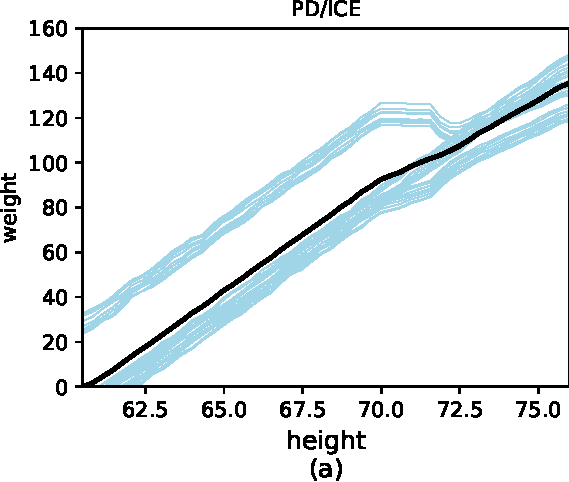
\includegraphics[scale=0.35]{images/height_vs_weight_pdp.pdf}~~
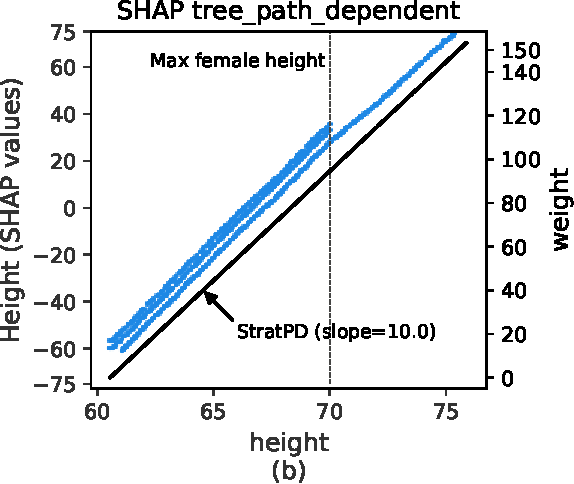
\includegraphics[scale=0.35]{images/weight_tree_path_dependent_shap.pdf}~~
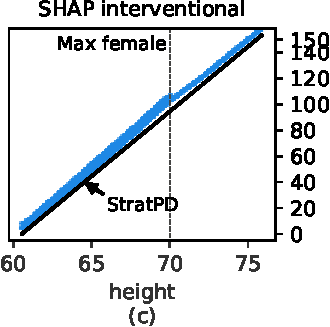
\includegraphics[scale=0.35]{images/weight_interventional_shap.pdf}~~
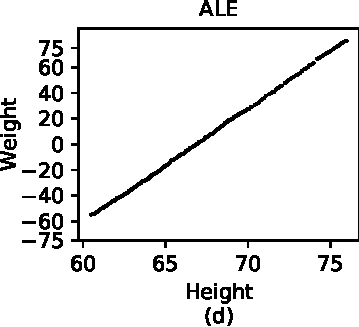
\includegraphics[scale=0.34]{images/height_ale.pdf}~~
\caption{\small SHAP partial dependence plots of response body weight on feature {\tt height} using 2000 synthetic observations from \eqref{eq:weight}. 50/50 male/female, half of the women are pregnant, and pregnancy contributes 40 pounds. SHAP interrogated an RF with 40 trees and explained 2000 samples; the interventional case used 100 observations as background data. RF OOB $R^2$ 0.999}
\label{fig:heightweight}
\end{center}
\end{figure}

\begin{figure}[htbp]
\begin{center}
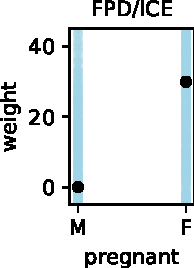
\includegraphics[scale=0.45]{images/pregnant_vs_weight_pdp.pdf}~~
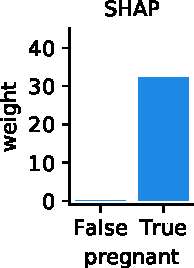
\includegraphics[scale=0.45]{images/pregnant_vs_weight_shap.pdf}~~
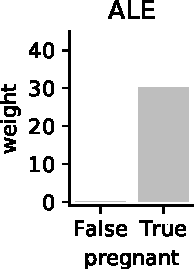
\includegraphics[scale=0.45]{images/pregnant_2_ale.pdf}~~
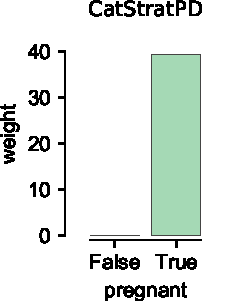
\includegraphics[scale=0.45]{images/pregnant_vs_weight_stratpd.pdf}~~
\caption{\small foo.}
\label{fig:pregnant}
\end{center}
\end{figure}

Even for experts, explaining this behavior requires some thought, and one must distinguish between model artifacts and interesting phenomena. The discontinuity at the maximum female height location arises partially from the model having trouble extrapolating for extremely tall pregnant women. Consider one of the upper ICE lines in \figref{fig:heightweight}(a) for a pregnant woman. As the ICE line slides $x_{height}$ above the maximum height for a woman, the model leaves the support of the training data and predicts a {\em lower} weight as height increases. ALE's curve is straight because it focuses on local effects, demonstrating that the lack of sharp slope-10 lines for FPD and SHAP cannot be attributed simply to a poor choice of model.  

SHAP also defines $x_j$ feature importance as the average magnitude of the $x_j$ SHAP values, which introduces a paradox.  The spread of the SHAP values alerts users to variable interactions, but allows contributions from other variables to leak in, thus, potentially leading to less precise estimates of $x_{height}$'s importance.

It is conceivable that a more sophisticated model (in terms of extrapolation) could sharpen the FPD and SHAP curves for $x_{height}$. There is a difference, however, between extrapolating to a meaningful but unsupported vector and making predictions for nonsensical vectors arising from variable codependencies.  Techniques that rely on such predictions make the implicit assumption of variable independence, introducing the potential for bias. Consider \figref{fig:pregnant} that presents the partial dependence results for categorical variable $x_{pregnant}$ (same data set). The weight gain from pregnancy is 40 pounds per \eqref{eq:weight}, but only \cspd{} identifies that exact relationship; FPD, SHAP, and ALE show a gain of 30 pounds. 

\cspd{} stratifies persons with the same or similar sex, education, and height into groups and then examines the relationship between $x_{pregnant}$ and $y$. If a group contains both pregnant and nonpregnant females, the difference in weight will be 40 pounds in this noiseless data set (assuming identical \xnj).  FPD and ALE rely on computations that require fitted models to conjure up predictions for nonsensical records, such as pregnant males (e.g., $\hat{f}(x_j = pregnant, {\bf X}_{\texttt{\char`\\}j})$). Not even a human knows how to estimate the weight of a pregnant male. SHAP, per its definition, does not require such predictions, but in practice for efficiency reasons, SHAP approximates $\Ex[\hat{f}(x_{j} = pregnant,{\bf X}_{\texttt{\char`\\}j}) | {\bf X}_j = x_j]$ with $\Ex[\hat{f}(x_{j} = pregnant,{\bf X}_{\texttt{\char`\\}j})]$, which does not restrict pregnancy to females. As discussed above, there are advantages to all of these model-based techniques, but this example demonstrates there is potential for partial dependence bias.

\cut{
pregnant female at max range [233.33467678]
pregnant female in male height range [228.71359869]
nonpregnant female in male height range [209.88006493]
male in male height range [219.46772083]
}


\cut{
$1/n*\sum_{i=1}^n f(x_j = pregnant, x_{i, \bar{j}}) - f(x_j = not pregnant, x_{i, \bar{j}})$

\noindent where ${x_{i, \bar{j}}: i=1,2,?,n}$ are the n training observations of $x_{\bar{j}}$
}

\begin{figure}[htbp]
\begin{center}
%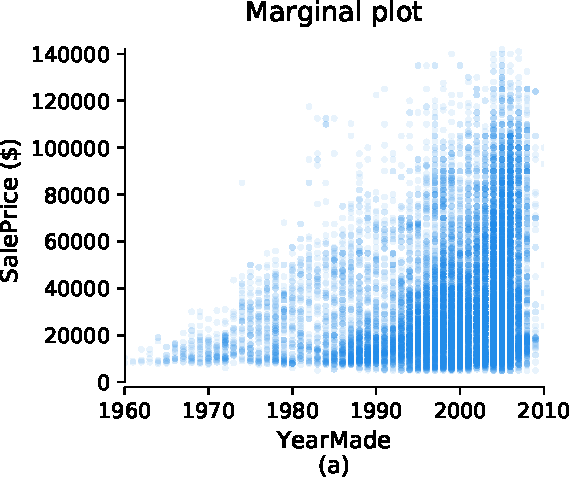
\includegraphics[scale=0.35]{images/bulldozer_YearMade_marginal.pdf}~~
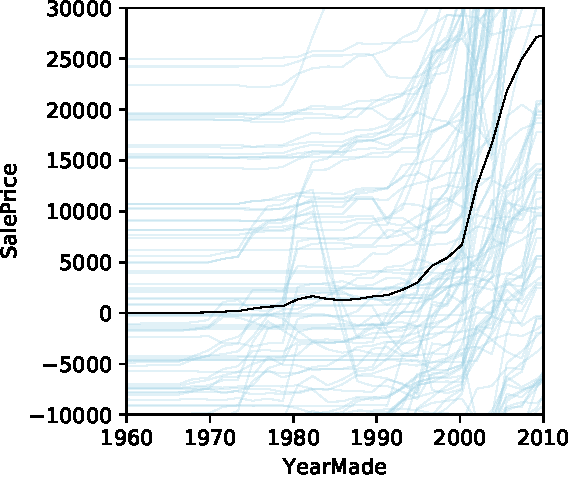
\includegraphics[scale=0.35]{images/bulldozer_YearMade_pdp.pdf}~~
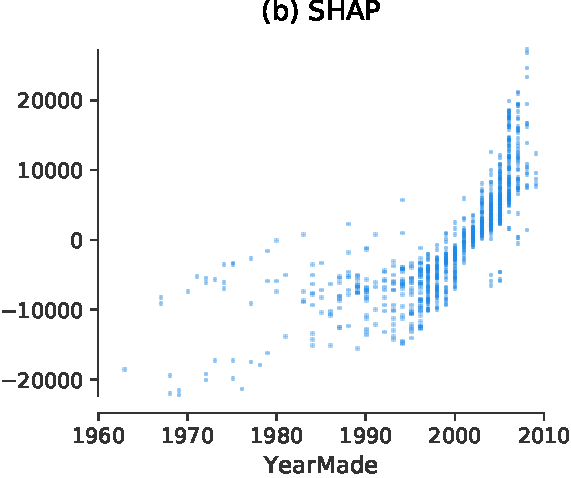
\includegraphics[scale=0.35]{images/bulldozer_YearMade_shap.pdf}~~
\includegraphics[scale=0.35]{images/YearMade_ale.pdf}~~
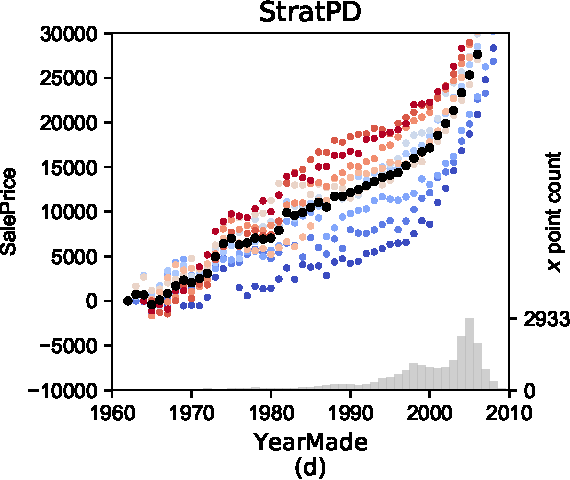
\includegraphics[scale=0.35]{images/bulldozer_YearMade_stratpd.pdf}
\caption{\small (a) Marginal plot of bulldozer {\tt YearMade} versus {\tt SalePrice} using subsample of 20k observations, (b) partial dependence drawn by SHAP interrogating an RF with 40 trees and explaining 1000 values with 100 observations as background data, (c) \spd{} partial dependence.}
\label{fig:yearmade}
\end{center}
\end{figure}


The stratification approach also gives plausible results for real data sets, such as the bulldozer auction data from \cite{bulldozer}. \figref{fig:yearmade} shows the partial dependence curves for the same set of techniques as before on feature {\tt\small YearMade}, chosen because it is very predictive of sale price. The shape and magnitude of the FPD, ALE, and \spd{} curves are similar, indicating that older bulldozers are worth less at auction, which is plausible. The \spd{} curve shows 10 bootstrapped trials where the heavy black dots represent the partial dependence curve and the other curves describe the variability.  The SHAP curve looks unexpectedly random, but the underlying mathematics are sound; perhaps this identifies an issue arising from performance compromises. (We have submitted an issue to their repo).

\cut{ % I'm just not sure this example is necessary and might be beating a dead horse
As a second example, consider the curves for feature {\tt\small MachineHours} in \figref{fig:machinehours}. As with bulldozer age, one would expect bulldozers with more use to cost less, but only the \spd{} curve shows that general trend.  Each plot shows some kind of visual phenomenon at 3138 hours, which coincides with a spike in the $x$ histogram of \figref{fig:machinehours}(d).  It would be easy to misinterpret this as an interesting feature of the data, but experts will recognize this as an artifact of data preparation.  A very common and effective technique is to replace missing values with the median (and add a ``is missing'' variable), as recommended by \cite{missingdata}.  Roughly 50\% of the {\tt\small MachineHours} values are missing and the dip at the median is because bulldozers with missing {\tt\small MachineHours} are, on average, worth less according to the training data (by about 4k\$).  The true relationship is unknown but the \spd{} plot seems the most plausible.

\begin{figure}[htbp]
\begin{center}
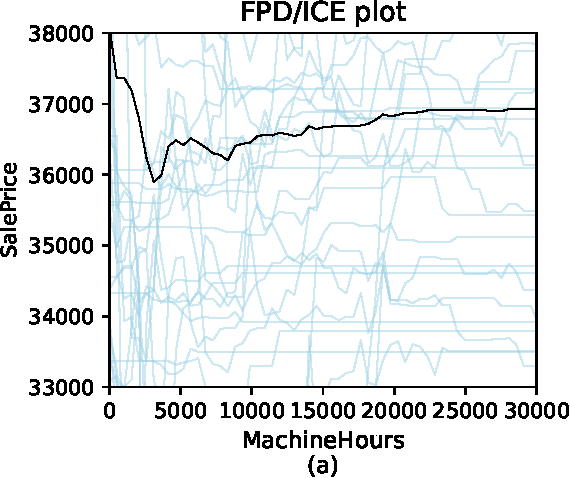
\includegraphics[scale=0.35]{images/bulldozer_MachineHours_pdp.pdf}~~
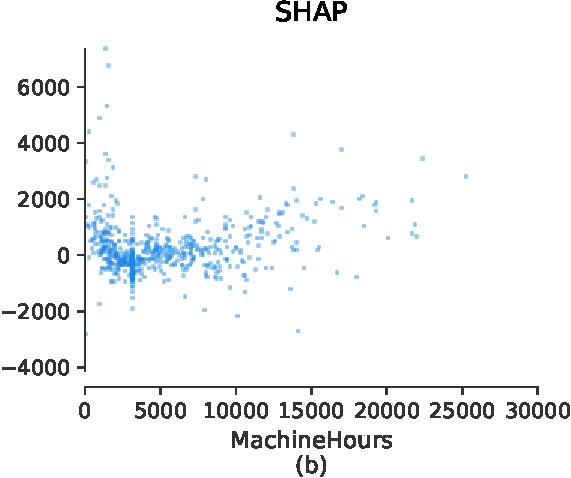
\includegraphics[scale=0.35]{images/bulldozer_MachineHours_shap.pdf}~~
\includegraphics[scale=0.35]{images/MachineHours_ale.pdf}~~
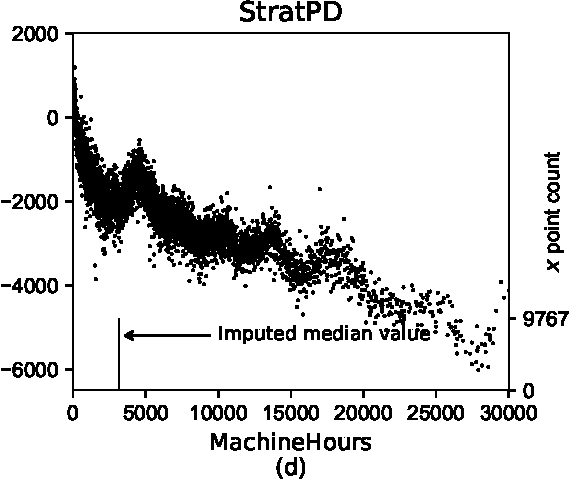
\includegraphics[scale=0.35]{images/bulldozer_MachineHours_stratpd.pdf}
\caption{\small (a) Marginal plot of bulldozer {\tt MachineHours} versus {\tt YearMade}.  bulldozers with MachineHours = 35,628 and without = 31,320. with and without YearMade: 2000.8 and 1998.6 so there is definitely a difference, on average, for those with and without machine hours listed. 4945 out of 10000 records have missing machine hours.  The dip at 3138 hours is the median. \spd{} is average of 10 trials bootstrapped}
\label{fig:machinehours}
\end{center}
\end{figure}
}

And, finally, an important consideration for any tool is performance, so we plotted execution time versus data size (up to 30,000 observations) for three real Kaggle data sets: rent, bulldozer, and flight arrival delays \cite{flights}. \figref{fig:timing} shows growth curves for 40 numerical variables and 11 categorical variables grouped by type of variable.  For these data sets, \spd{} takes 1.1s or less to process 30,000 records for any $x_j$, despite the potential for quadratic cost. \cspd{} typically processes categorical variables in less than 2s but takes 13s for the high-cardinality categorical {\tt\small ModelID} of bulldozer (which looks mildly quadratic).  These elapsed times for our prototype show it to be practical and competitive with FPD/ICE, SHAP, and ALE.  If the cost to train a model using (cross validated) grid search for hyper parameter tuning is included, \spd{} and \cspd{} outperforms these existing techniques (as training and tuning is often measured in minutes).

\begin{figure}[htbp]
\begin{center}
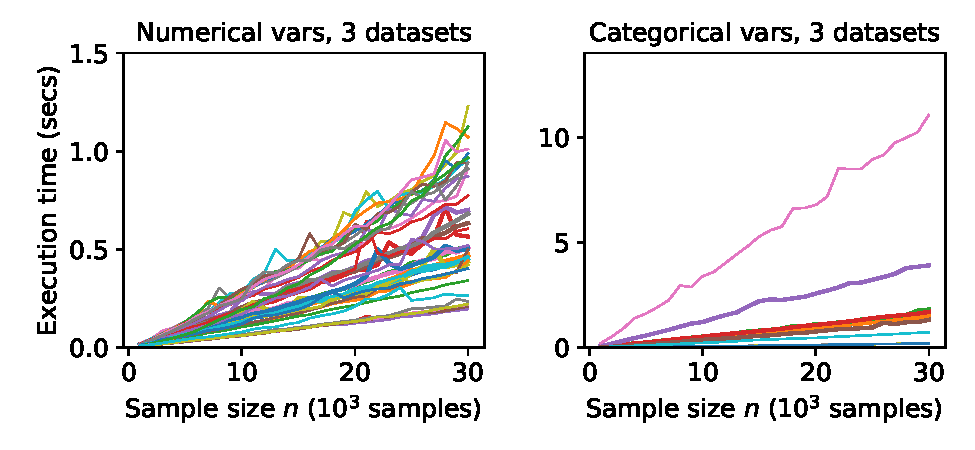
\includegraphics[scale=.4]{images/timing.pdf}
\caption{\small timing blah. $p=20$, bulldozer $p=14$, and flight $p=17$. Numba JIT warmup Numba just-in-time compiler ({\tt\small numba.pydata.org})}
\label{fig:timing}
\end{center}
\end{figure}

what if X,y relationship is very weak? models would get low accuracy. what happens to us?  I think we would simply show low partial dependence curves.

\todo{unsupervised?}

\cut{
flight shape (5714008, 17), 6 cats
rent shape (49352, 20), no cats
bulldozer shape (362781, 14) records, 5 cats
}

All simulations in this section were run on a 4.0 Ghz 32G RAM machine running OS X 10.13.6 with SHAP 0.34, scikit-learn 0.21.3, XGBoost 0.90, and Python 3.7.4.

% ------------------------------------------------------------------------------------------------------------------------------------
\section{Discussion and future work}

can parallelize code or do in C++.

similar to ALE but much simpler for categorical variables.

we can handle partial derivatives for $x_{j,l}$ using 2D finite difference to get gradients then using double integral instead of single cumulative sum. I believe that gets us an estimate for plot value at point ($x_j, x_l$).  actually looks like the ALE guy is calling it a second order effect and is subtracting the two one-dimensional finite differences. Hmm... he's just holding $x_j, x_l$ constant and integrating over the other variables to find the value at $(x_j, x_l)$.
 
it couldn't handle it when I got rid of education in  body weight data set. got 0 pdpy. perhaps investigate

A word on hyper parameters. All techniques have hyper parameters that can affect results, particularly if one includes hyper parameters in the model itself for model-based techniques.  For example, a SHAP plot like \figref{fig:yearmade}(c) with fewer explained vectors looks much more like a line but then does not alert the user about variable interactions.  It is sound practice to try a variety of hyper parameters with any partial dependence technique, including ours.

Our goal here is not to say these other techniques are not useful. Rather, we are pointing out potential issues and hoping to open a new line of inquiry that experiments have shown to be accurate in cases where previous techniques are not.

% ------------------------------------------------------------------------------------------------------------------------------------
\section{Appendix}

\cut{
\begin{alltt}
{\fontfamily{cmss}\selectfont\small
{\bf{}StratPD}
\(T\) = Tree regressor fit to \xnj with hyper parameter {\tt{}min_samples_leaf}
For each leaf in \(T\):
    \(\bf\overline{y}\) = Group leaf samples by \(x\sb{j}\), computing average \(y\) per unique \(x\sb{j}\)
    {\bf{}dx} = discrete difference between adjacent unique \(x\sb{j}\) values
    {\bf{}dy} = discrete difference between adjacent average \(\bf\overline{y}\) values
    add (x[i], x[i+1], dy[i]/dx[i]) for each unique \(x\sb{j}\) to list D
For each \(x\) in unique \({\bf{}X}\sb{j}\):
    slopes = [\(slope\) for (\(a, b, slope\)) in D if \(x \ge a\) and \(x < b\)]
    count[x] = |slopes|
    dydx[x] = mean(slopes)
Drop slope estimates computed using fewer than {\tt{}min_slopes_per_x values}
pdx = discrete difference between adjacent unique \(x\sb{j}\)
pdy = cumulative sum of dydx * pdx
return pdx, [0]+pdy  // insert 0 for pdx[0] since sum contributed from beyond left is 0
}
\end{alltt}
}

\SetAlgoNoEnd%
\setlength{\algomargin}{5pt}
\begin{algorithm}[H]
\SetAlgoLined
\DontPrintSemicolon
\SetAlgorithmName{Algorithm}{List of Algorithms}
\SetAlgoSkip{}
\TitleOfAlgo{{\em StratPD}({\bf X}, {\bf y}, $j$, {\it min\_samples\_leaf}, {\it min\_slopes\_per\_x})}
\small
$T$ := Decision tree regressor fit to (\xnj{}, $\bf y$) with hyper parameter: ${\it min\_samples\_leaf}$\;
\For{each leaf $L \in T$}{
        $({\bf x}_L, {\bf y}_L)$ := $\{(x_j^{(i)},  y^{(i)})\}_{i \in L}$\Comment*{\it Get leaf observations}
	${\bf ux}, \bar{\bf y}$ := Group and sort $({\bf x}_L, {\bf y}_L)$ by $x_j$ value, computing $\bar{y}$ per unique $x_j$ value\\
	${\bf dx}$ := ${\bf ux}^{(i+1)} - {\bf ux}^{(i)}$ for $i = 1..|{\bf ux}|-1$\Comment*{\it Discrete difference between adjacent}
	${\bf dy}$ := $\bar{\bf y}^{(i+1)} - \bar{\bf y}^{(i)}$ for $i = 1..|{\bf ux}|-1$\\
	Add tuples ${({\bf ux}^{(i)}, {\bf ux}^{(i+1)},~ {\bf dy}^{(i)}/{\bf dx}^{(i)})}$  to list ${\bf D}$ for $i = 1..|{\bf ux}|-1$\\
}
$\bf ux$ := $unique({\bf X}_j)$\\
\For(\hfill$\triangleright$\ {\it\textcolor{gray}{\small Count slopes and compute average slope per unique $x_j$ value}}){each $x \in {\bf ux}$}{
	{\bf slopes} := [$slope$ for $(a,b,slope) \in \bf D$ if $x \ge a$ and $x <b$]\\
	${\bf c}_x$ := $|{\bf slopes}|$\\
	${\bf dydx}_x$ := $\overline{\bf slopes}$\\
}
${\bf dydx}$ := ${\bf dydx}[{\bf c} \ge min\_slopes\_per\_x]$\Comment*{\it Drop missing slopes, those computed with too few}
${\bf ux}$ := ${\bf ux}[{\bf c} \ge min\_slopes\_per\_x]$\\
$\bf pdx$ := ${\bf ux}^{(i+1)} - {\bf ux}^{(i)}$ for $i = 1..|{\bf ux}|-1$\\
$\bf pdy$ := [0] + cumulative\_sum(${\bf dydx} * \bf pdx$)~~~\Comment*{\it integrate, inserting 0 for leftmost $x_j$}
\Return{$\bf pdx, pdy$}
\label{alg:StratPD}
\end{algorithm}

\cut{
\begin{alltt}
{\fontfamily{cmss}\selectfont\small
{\bf{}CatStratPD}
Fit tree regressor to all but \(x\sb{j}\) with hyper parameter min_slopes_per_x
For each leaf:
    y bar = Group leaf samples by categories of \(x\sb{j}\), computing average y per unique category \(x\sb{j}\)
    Compute unique categories and counts per category
    refcat is randomly chosen category from \(x\sb{j}\)
    For each unique category x in leaf:
        delta[cat,leaf] = Subtract y for refcat from all y bar (refcat delta will be 0)
end
Let Avg[cat] be vector with running sum mapping category to count
work = set of leaf indexes
while more work and something changed and less than max iterations:
    for each leaf in leaves:
        if cat in delta[:,leaf] intersects with Avg:
            j = random category in intersection
            adjust delta[:,leaf] to be relative to j so delta[j,leaf]==0 then add Avg[j] so comparable
            merge into Avg
    work -= all j merged this iteration
}
\end{alltt}
}

\setlength{\algomargin}{5pt}
\begin{algorithm}[H]
\SetAlgoLined
\DontPrintSemicolon
\SetAlgorithmName{Algorithm}{List of Algorithms}
\SetAlgoSkip{}
\TitleOfAlgo{{\em CatStratPD}(${\bf X}, {\bf y}, j, {\it min\_samples\_leaf}$)}
\small
\cut{
\KwOut{$\begin{array}[t]{l}
\Delta^{(k)} = \text{category } k \text{'s effect on } y \text{ where } mean(\Delta^{(k)})=0\\
n^{(k)} = \text{number of supported observations per category $k$}\\
\end{array}$
}
}
$T$ := Decision tree regressor fit to (\xnj{}, $\bf y$) with hyper parameter: ${\it min\_samples\_leaf}$\;
Let $\Delta Y$ be a matrix whose columns are vectors of leaf category deltas\\
Let $C$ be a matrix whose columns are vectors for leaf category counts\\
\For(\hfill$\triangleright$\ {\it\textcolor{gray}{\small Get average $y$ delta relative to random ref category for obs. in leaves}}){each leaf $L \in T$}{
        $({\bf x}_L, {\bf y}_L)$ := $\{(x_j^{(i)},  y^{(i)})\}_{i \in L}$\Comment*{\it Get leaf observations}
        ${\bf ucats}$, $C_L$ := $unique({\bf x}_L)$\Comment*{\it Get unique categories, counts from leaf observations}
	$\bar{\bf y}$ := Group leaf records $({\bf x}_L, {\bf y}_L)$ by category, computing $\bar{y}$ per unique category\\
	${\it refcat}$ := random category from ${\bf x}_L$\\
%	$y_{\it ref}$ := random choice from $\bar{\bf y}$\\
	$\Delta {Y}_L$ = $\bar{\bf y} - \bar{\bf y}_{\it refcat}$\\
}
$\Delta {\bf y}$, {\bf c} := $\Delta {Y}_1$, $C_1$\Comment*{\it $\Delta {\bf y}$ is running average vector mapping category to average $y$ delta}
$completed$ := $\{1\}$; $work$ := $\{2 .. |leaves|\}$; \Comment*{\it set of leaf indexes}
%${\bf ucats}$ := $unique({\bf X}_j)$\\
\While(\hfill$\triangleright$\ {\it\textcolor{gray}{\small 2 passes is typical to merge all $\Delta {Y}_L$ into $\Delta {\bf y}$}}){$|work| > 0$ and $|completed|>0$}{
    completed := $\emptyset$\\
    \For{each leaf $L$ in work}{
        \If{$\Delta {Y}_L$ has category in common with $\Delta {\bf y}$}{
            ${\it completed}$ := ${\it completed} \cup \{L\}$\\
            $c$ = random category in intersection\\
            $\Delta {\bf y}_L$ := $\Delta {Y}_L- \Delta {Y}_{L,{\it c}} + \Delta {\bf y}_{\it c}$\Comment*{\it Adjust so $\Delta {Y}_{L,{\it c}}=0$, add corresponding $\Delta {\bf y}_{\it c}$ value}
            $\Delta {\bf y}$ := $({\bf c} \times \Delta {\bf y} + C_L \times \Delta {\bf y}_L)/({\bf c} + C_L)$ where $z+NaN$={\it z}\Comment*{\it weighted average}
            ${\bf c} := {\bf c} + C_L$\Comment*{\it update running weight}
        }
    }
    $work := work \texttt{\char`\\} {\it completed}$\\
}
\Return{$\Delta {\bf y}$}\\
\label{alg:CatStratPD}
\end{algorithm}


{\small
\bibliography{stratpd}
}
\end{document}